\documentclass[11pt, a4paper]{article}
\usepackage{geometry}
\usepackage{amsmath,amssymb}
\usepackage{booktabs}
\usepackage{pdflscape}
\usepackage{graphicx}
\usepackage{array}
\usepackage{amsmath}
\usepackage{floatrow}
\usepackage{upquote}
\usepackage[pdftex,unicode]{hyperref}
\usepackage{extsizes}
\usepackage{xcolor}
\usepackage{subfigure}
\usepackage{dcolumn}
\usepackage{float}
\usepackage{lscape}
\usepackage{rotating}
\usepackage{refstyle}
\usepackage{enumerate}
\usepackage{amsmath}
\usepackage{amssymb}
\usepackage[parfill]{parskip}
\usepackage{apacite}
\usepackage{fancyhdr}
\usepackage[czech]{babel}
\usepackage{listings}
%\usepackage{tikz}
\usepackage[utf8]{inputenc}
\usepackage[T1]{fontenc}
\usepackage{lmodern}
\usepackage[svgnames]{xcolor}
\usepackage{setspace}
\onehalfspacing  
%\doublespacing


\geometry{includefoot, left=3cm, right=3cm, top=2.8cm, bottom=2.0cm}
\setlength{\parindent}{0em}
\setlength{\parskip}{1em}
\newcommand{\forceindent}{\leavevmode{\parindent=2cm\indent}}

%\hypersetup{pdfstartview={XYZ null null 1.00}}
%\linespread{1.25}
\pagestyle{fancy}
\begin{document}

\begin{titlepage}
\begin{center}
\vspace*{1cm}

\Huge
Praktikum z Ekonometrie

\vspace{0.5cm}
\LARGE
Prostorové modely na trhu Pražských bytů

\vspace{2.5cm}

Petr Hrobař

\vfill

Seminární práce

\vspace{0.8cm}

\includegraphics[width=0.4\textwidth]{university}

\Large
Vysoká škola ekonomická v Praze\\

\end{center}
\end{titlepage}


\clearpage

\tableofcontents

\clearpage

\section{Úvod}

V této seminární práci budeme aplikovat prostorové modely na trhu pražských bytů. Uvažujeme, že cena není pouze funkcí vlastních charakteristik každé nemovitosti, ale také funkcí lokality. V návaznosti na \textit{Toblerovo pravidlo geografie:} o podobnosti sousedních jednotek, modelujeme cenu nejen jako funkci vlastních charakteristik, ale také charakteristik sousedních jednotek. 

Poznatky naší studii jsou následující: Nejdříve na základě parametru prostorové autokorelace (statisticky signifikantní na 1\% hladině) potvrzujeme prostorovou závislost, tj, že ceny pražských nemovitostí nejsou náhodně rozmístěny v prostoru, ale tvoří určité \textit{prostorové clustery}, kde ceny a charakteristiky nemovitostí jsou si více podobné, než mimo ně. 

Dále jakmile bereme v potaz prostorovou závislost, jsme schopni ceny nemovitostí odhadovat přesněji. Nakonec dle distribuce reziduí identifikováváme \textit{honosné clustery}, kde cena nemovitostí může být i dvojnásobně vetší než její predikce, čistě z důvodů lokality.

Formálně si stanovíme následující výzkumné hypotézy:
  
  \begin{itemize}
\item H{1}: \textit{Z důvodu prostorové autokorelace disponují prostorové modely lepší predikční schopnosti.}

\item H{2}: \textit{Historické centrum Prahy představuje hlavní „honosný“ cluster.}

\item H{3}: \textit{Novostavba výrazně zvýší cenu}
\end{itemize}

\section{Dataset}

Kompletní dataset získaný pro analýzu pochází z internetových stránek realitní kanceláře \url{www.sreality.cz}. Vlastní data byly extrahovaná z webu dne 10. března 2020 využitím techniky \textit{webscrapingu} v programovacím jazyku PYTHON. V případě zájmu je dataset a výpočetní kódy k dispozici u autora seminární práce. 

Z webu bylo extrahováno více než 5 000 záznamů o více než 100 proměnných. Pro účely naší analýzy bylo nutné proměnné, které nejsou pro naší analýzu relevantní, vyjmout. Dataset tedy obsahuje pro každou nemovitost následující proměnné: \textit{Cena (price), Počet pokojů (Rooms), Metry čtverečný (Meters), Mezonový byt (Mezone), Kuchyňský koutek (KK), Panelový typ (Panel), Balkón/Terasa (balcony or terrase), Novostavba (Novostavba), Souřadnice.} 

Dále bylo nezbytné odstranit všechna pozorování, která obsahovala neúplné záznamy ve výše vypsaných proměnných. Celkem datový soubor obsahuje 2 984 kompletních záznamů.

\subsection{Základní charakteristiky}

V rychlosti nahlédněme na popisné statistiky našich proměnných. Jednotlivé relevantní statistiky josu popsány v tabulce \ref{Popisné statistiky proměnných} níže:
  
  \begin{table}[!htbp] \centering 
\caption{Popisné statistiky proměnných} 
\label{Popisné statistiky proměnných} 
\scalebox{0.75}{
  \begin{tabular}{@{\extracolsep{5pt}}lccccccc} 
  \\[-1.8ex]\hline 
  \hline \\[-1.8ex] 
  Statistic & \multicolumn{1}{c}{N} & \multicolumn{1}{c}{Mean} & \multicolumn{1}{c}{St. Dev.} & \multicolumn{1}{c}{Min} & \multicolumn{1}{c}{Pctl(25)} & \multicolumn{1}{c}{Pctl(75)} & \multicolumn{1}{c}{Max} \\ 
  \hline \\[-1.8ex] 
  price & 2,984 & 8,495,653.000 & 5,696,973.000 & 80,000 & 4,990,000 & 9,990,000 & 79,000,000 \\ 
  Rooms & 2,984 & 2.804 & 1.128 & 1 & 2 & 4 & 6 \\ 
  Meters & 2,984 & 79.634 & 40.968 & 15 & 52 & 96 & 435 \\ 
  Mezone & 2,984 & 0.027 & 0.163 & 0 & 0 & 0 & 1 \\ 
  KK & 2,984 & 0.792 & 0.406 & 0 & 1 & 1 & 1 \\ 
  panel & 2,984 & 0.132 & 0.338 & 0 & 0 & 0 & 1 \\ 
  balcony\_or\_terrase & 2,984 & 0.514 & 0.500 & 0 & 0 & 1 & 1 \\ 
  metro & 2,984 & 0.979 & 0.143 & 0 & 1 & 1 & 1 \\ 
  novostavba & 2,984 & 0.291 & 0.454 & 0 & 0 & 1 & 1 \\ 
  \hline \\[-1.8ex] 
  \end{tabular} }
\end{table} 

Dále také testujeme jednotlivé vysvětlující proměnné na výraznou korelaci mezi sebou, abychom dodrželi předpoklad na absenci \textit{dokonalé multikolinearity}. Je zřejmé, že lze předpokládat výraznou korelaci mezi proměnnými \textit{Meters a Rooms}. Uvažujeme ale, že proměnné nejsou \textit{dokonale korelované}\footnote{Tato korelace nabývá hodnoty \textit{0.726}.} a do modelů budeme využívat obě.  

Dále lze nahlédnout na histogramy proměnných na obrázku \ref{Distribuce Proměných} v sekci \ref{Přílohy}. Distribuce proměnných v prostoru je možné sledovat na obrázku \ref{Distribuce pozorování v prostoru} v sekci \ref{Přílohy}.

\section{Metodologie}
\subsection{Využitý model}

K ověření našich stanovených hypotéz sestavíme model, který bude mít následující podobu:
  \begin{equation} \label{rovnice1}
log(price) = \beta_{0} +  \beta_{1}rooms  + \beta_{2}log(meters) + \beta_{3}mezon + \beta_{4}kk + \beta_{5}panel + \beta_{6}terasa/balkon + \beta_{7}novostavba + \varepsilon.
\end{equation}

Z histogramů proměnných\ref{Distribuce Proměných} lze usuzovat, že proměnné \textit{Price} a \textit{Meters} pocházejí z \textit{log-normálního rozdělení} tj, že logaritmus proměnné má rozdělení \textit{normální.} Obě proměnné tedy logaritmujeme. Tato forma modelů také poslouží k potlačení případně \textit{heteroskedasticity} a lepšímu popisu vztahů v proměnných.

Model \ref{rovnice1} budeme odhadovat několika metodami: \textit{Metody nejmenších čtverců (OLS), Kvantilová regrese, Spatil lag model, Spatial error model.}

\subsection{Základní modely}
\subsubsection{OLS model}

V rychlosti připomeňme regresi s využitím metody nejmenších čtverců. Minimalizujeme kvadráty reziduí dle vzorce:
  $$RSS = \sum_{i = 1}^{n} \Big(y_{i} - \beta_{0} - \sum_{j = 1}^{p}\beta_{j}x_{ij}\Big)^2, $$
  
  Kde řešení je k dispozici v analytickém tvaru:
  $$\hat\beta = (X^{T}X)^{-1}X^{T}y.$$
  
  U čtenářů očekáváme pokročilou znalost metody OLS a nebude zde opakovat podrobné vlastnosti a předpoklady odhadu. Pro rychlou rekapitulaci lze odkázat na literaturu např. \cite{wooldridge2016introductory-citovat_kapitolu}.

Dále abychom vzali částečně v potaz prostorovou závislost využijeme proměnných \textit{souřadnic}. Obě proměnné není vhodné přímo vložit do modelu, ale lze využit Clusterovacího algoritmu a následně do modelu vložit identifikátor Clusteru. Pro naší studii využijeme \textit{k-means} algoritmu \cite{james2013introduction}. Pro ilustraci fungování Clusterování souřadnic lze nahlédnout na obrázek \ref{Distribuce Pozorování a Clusterování}. Do modelu bude následně vložena Dummy proměnná každého Clusteru. Pokud proměnné identifikátoru \textit{Clusteru} budou signifikantní, lze toho využít jako určitého indikátoru \textit{prostorového shluku}.

\subsubsection{Kvantilová regrese}
Metoda kvantilové regrese regrese, je metoda ve které se minimalizuje následující tvar:
  
  každé $i-$té reziduum má podobu:
  $$e_{i} = (y_{i} - x_{i}\hat\beta_{q}), $$
  pro každý konkrétní $q-$tý kvantil odhadujeme parametry $\hat \beta_{q}$ takové, aby se minimalizoval výraz:
  
  $$min: Q_{n}(\hat\beta_{q}) = \sum_{i:\ e_{i}\geq 0}^{n} q|y_{i} - x_{i} \hat\beta_{q}| + \sum_{i:\ e_{i}	\leq 0}^{n} (1-q)|y_{i} - x_{i} \hat\beta_{q}|.$$
  
  Řešení výše není k dispozici v analytickém tvaru a úloha se řeší iteračně jako úloha lineárního programování \cite{greene2003econometric}.

Je dobře známo, že metoda je robustní vůči odlehlým pozorováním. Jelikož náš datový soubor také obsahuje velké množství pozorování (\textit{n = 2 984}) lze očekávat vhodné asymptotické vlastnosti. Abychom také ověřili stabilitu koeficientů pro různé hodnoty kvantilů. Provedeme regresi pro jednotlivé decily datového souboru.

\subsection{Prostorové modely}
Než začneme aplikovat prostorové modely, je nezbytné ověřit prostorovou autokorelaci. Standartní testy pro přítomnost prostorové autokorelace ověřují souvislosti mezi polohou pozorování hodnotami proměnných. 

Výhodou prostorových modelů je možnost kontroly prostorové závislosti v data generujícím procesu (DGP). Nicméně, aby bylo možné statistické inference a odhady koeficientů byly co nejpřesnější, je nezbytné korektní specifikování prostorové závislosti.

\subsubsection{Spatil lag model}

\textit{Spatil lag} model bere v potaz prostorovou závislost mezi vysvětlujícími proměnnými. Formálně lze model přepsal do podoby:
  
  \begin{equation} \label{spatial lag}
y = \rho W y + X\beta + \varepsilon, 
\end{equation}

Kde parametr \textit{$\rho$} představuje parametr prostorové autokorelace. Z předpisu je patrné, že pokud: \textit{$\rho = 0$}, pracujeme s běžným OLS modelem. Řešení \ref{spatial lag} není k dispozici v analytickém tvaru a jako odhadová metoda parametrů modelu se užívá metoda \textit{maximální věrohodnosti}. Pro vetší detaily lze nahlédnout např. \cite{lesage2008introduction}, \cite{formanek2019spatial}.

Dále parametr \textit{W} představujeme \textit{matici sousednosti.}. Jedná se o matici o rozměru \textit{$n \times n$}, která udává, která pozorování jsou definována jako sousední a která nikoliv. Matice sousednosti \textit{W} představuje hlavní prvek prostorové ekonometrie \cite{lesage2008introduction}. Jelikož dochází k nadefinování matice před samotným odhadem modelu je nezbytná její korektní specifikace. 

Mezi nejčastější metody nadefinování relace sousednosti lze zmínit metodu: \textit{K-nejbližších sousedů, Maximální vzdálenost} a v případě pozorování v rámci regionů nebo zemí, kdy pracujeme s \textit{Polygony} také metody \textit{Rook} a \textit{Queen} sousednosti. Tím se dostáváme zpět k problematice testování prostorové autokorelace, korektní nadefinování sousednosti je nezbytné, neboť matice \textit{$W$} vstupuje také do testů prostorové autokorelace.


\subsubsection{Spatial Error model}
Model typu \textit{Spatial error} bere v potaz prostorovu závislost náhodně složky modelu a né proměnou vysvětlující. Formálně lze model zapsat do následující podoby:
  
  \begin{equation} \label{spatial error}
y = X\beta + u, 
\end{equation}
\begin{equation*}
u = \lambda W u + \varepsilon,
\end{equation*}

U modelu můžeme opět testovat zda parametr \textit{$\lambda$} nabývá hodnoty různé od $0$. Pokud by parametr nabýval hodnoty $0$, výraz zmizí a opět pracujeme se základním OLS modelem. Stejně jako u \textit{Spatial Error} modelu není řešení modelu \ref{spatial error} k dispozici v analytickém tvaru a opět užíváme metody \textit{maximální věrohodnosti}, kde maximalizujeme \textit{věrohodnostní funkci.} Pro rychlou revizi metody maximální věrohodnosti lze nahlédnout do \cite{wooldridge2016introductory-citovat_kapitolu}. Pro Detailnější popis prostorové spatial error modelu lze nalézt v  \cite{james2013introduction}, \cite{formanek2019spatial}. Výhodu modelu je, že koeficienty lze interpretovat, jako mezní efekty.


\subsubsection{Prostorová autokorelace a relace sousednosti}

Mezi nejužívanější test prostorové autokorelace patří \textit{Moranův I test} \cite{lesage2008introduction}, který lze zapsat následovně:
  
  \begin{equation}
I = \frac{n}{\sum_{i}\sum_{j}w_{ij}} \times \frac{\varepsilon^{'} W \varepsilon}{\varepsilon^{'} \varepsilon},
\end{equation}

kde \textit{$n$} je počet pozorování, \textit{$w_{ij}$} představuje prvky matice \textit{$W$}, dále \textit{$\varepsilon$} představuje vektor reziduí z OLS modelu.

V případně nulové hypotézy o prostorové nezávislosti nabývá statistika:
  
  \begin{equation}
E(I_{0}) = \frac{-1}{n-1,}
\end{equation}

V simulačních experimentech se \textit{Moranův test} prokazatelně odlišoval s ostatními testy v kontextu přesnosti  \cite{anselin2013spatial}. Relace sousednosti můžeme také nadefinovat prvotně na základě úvahy. 

\clearpage
Jelikož modelujeme ceny nemovitostí a předpokládáme, že ceny se vzájemně ovlivňují lokálně, uvažujeme, že sousední nemovitosti o stejných charakteristikách budou mít podobnou cena, která bude také zahrnovat faktor lokality. 

Budeme tedy vytvářet relaci sousednosti dle \textit{Počtu nejbližších sousedů}. Prvotně volíme hodnotu \textit{$k = 7$}.

Matice sousednosti může být vizualizována jako relace sousednosti pro každou pozorovanou jednotku v prostoru. Nahlédněme na relaci sousednosti na obrázku \ref{Relace sousednosti}:
  
  \begin{figure}[ht]
\label{}
\centering
\noindent\makebox[\textwidth]{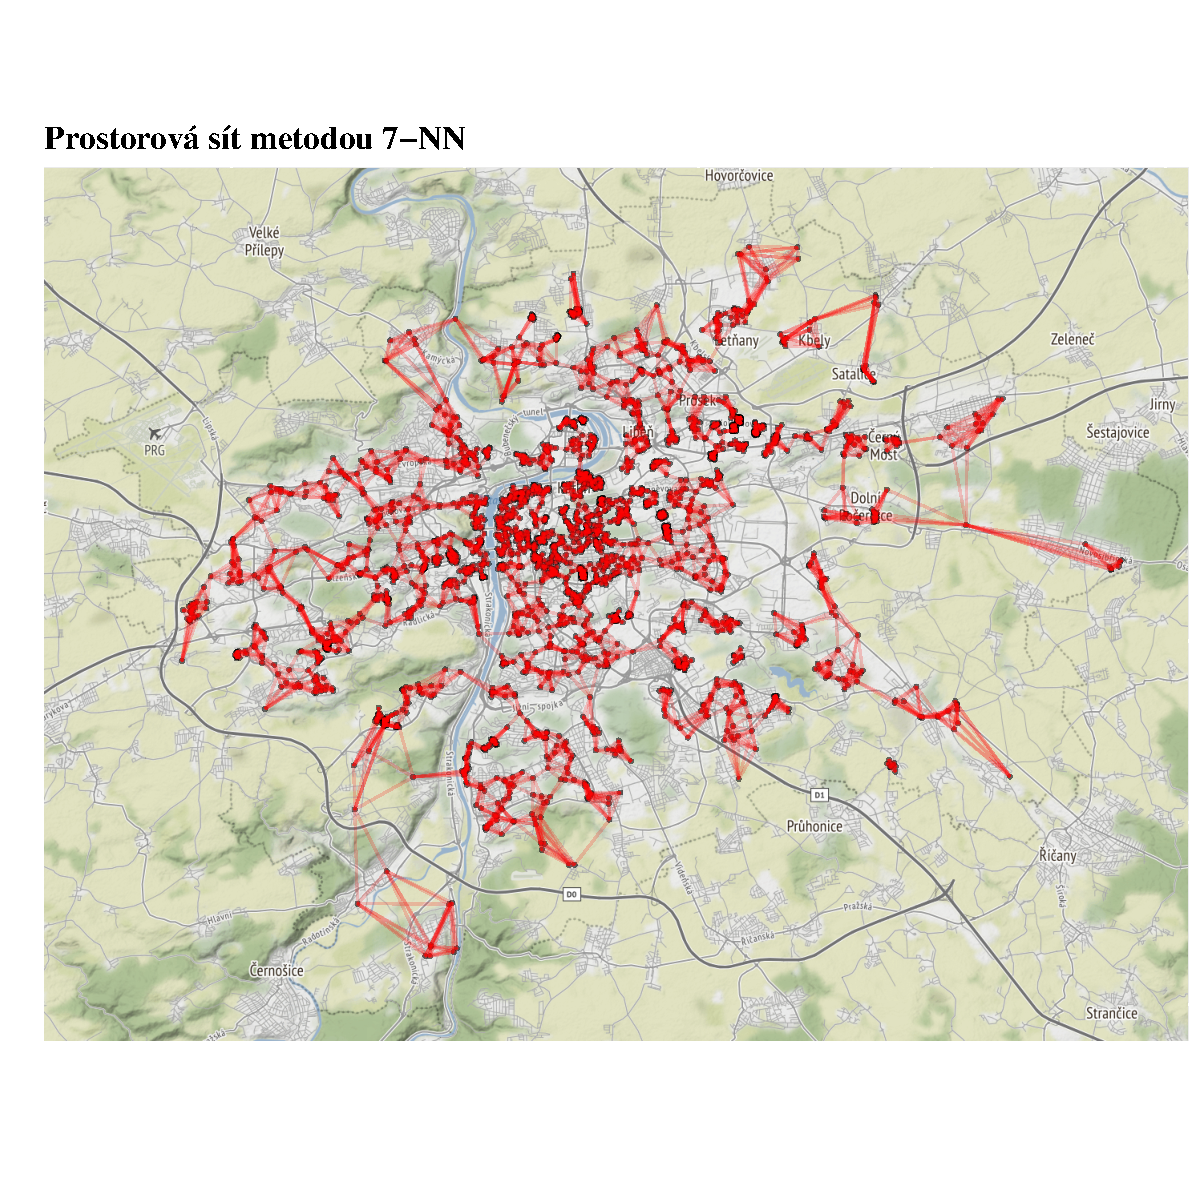
\includegraphics[width=1.15\textwidth]{flats_network.pdf}}
\caption{Relace sousednosti (\textit{7 nejbližších sousedů})}
\label{Relace sousednosti}
\end{figure}

Následně pro zvolenou relaci sousednosti provedeme \textit{Moranův Test}, formální test a jeho výstup je možné sledovat v tabulce \ref{Moran}:
  \clearpage

\begin{table}[!htbp] \centering 
\caption{Moranův Test 7-NN} 
\label{Moran} 
\scalebox{0.9}{
  \begin{tabular}{@{\extracolsep{5pt}} cccc} 
  \\[-1.8ex]\hline 
  \hline \\[-1.8ex] 
  & \textit{I-}statistika & Rozptyl & p-value \\ 
  \hline \\[-1.8ex] 
  & $0.413$ & $0.0001$ & $0.000$ \\ 
  \hline \\[-1.8ex] 
  \end{tabular} }
\end{table} 

je patrné, že v data generujícím procesu se vyskytuje statisticky signifikantní prostorová autokorelace a volíme metodiku prostorových modelů. 

O prostorové závislosti lze také uvažovat dle OLS modelů s \textit{Kmeans} proměnnou v tabulce \ref{modely tabulka}, kde proměnné Clusterů jsou statisticky signifikantní. 


\section{Empirická část}

Výše v  rychlosti popisujeme všechny modely a modifikace, které budeme v naši studii využívat, odhady dílčích koeficientů všech modelů je možné sledovat v tabulce \ref{modely tabulka}:
  
  \begin{table}[!htbp] \centering 
\caption{Odhady všech modelů} 
\label{modely tabulka} 
\scalebox{0.7}{
  \begin{tabular}{@{\extracolsep{5pt}}lcccccc} 
  \\[-1.8ex]\hline 
  \hline \\[-1.8ex] 
  & \multicolumn{6}{c}{\textit{Vysvětlovaná proměnná:}} \\ 
  \\[-1.8ex] & \multicolumn{6}{c}{\textit{log(price)}} \\ 
  \\[-1.8ex] & \multicolumn{2}{c}{\textit{OLS}} & \multicolumn{2}{c}{\textit{quantile}} & \multicolumn{2}{c}{\textit{Prostorové}} \\ 
  & \multicolumn{2}{c}{\textit{}} & \multicolumn{4}{c}{\textit{}} \\ 
  &  & \textit{k-means} &   & \textit{K-means} & \textit{Spatial Lag} & \textit{Spatial Error} \\ 
  \\[-1.8ex] & (1) & (2) & (3) & (4) & (5) & (6)\\ 
  \hline \\[-1.8ex] 
  \textit{Rooms} & 0.061$^{***}$ & 0.082$^{***}$ & 0.053$^{***}$ & 0.089$^{***}$ & 0.081$^{***}$ & 0.082$^{***}$ \\ 
  & (0.010) & (0.009) & (0.009) & (0.008) & (0.007) & (0.007) \\ 
  \textit{log(Meters)} & 0.808$^{***}$ & 0.731$^{***}$ & 0.818$^{***}$ & 0.692$^{***}$ & 0.667$^{***}$ & 0.685$^{***}$ \\ 
  & (0.021) & (0.019) & (0.019) & (0.018) & (0.017) & (0.016) \\ 
  \textit{Mezone} & $-$0.003 & $-$0.032 & 0.0001 & $-$0.041 & -0.048$^{*}$ & $-$0.067$^{**}$ \\ 
  & (0.031) & (0.027) & (0.022) & (0.027) & (0.025) & (0.023) \\ 
  \textit{KK} & 0.117$^{***}$ & 0.162$^{***}$ & 0.095$^{***}$ & 0.157$^{***}$ & 0.160$^{***}$ & 0.176$^{***}$ \\ 
  & (0.016) & (0.014) & (0.017) & (0.013) & (0.012) & (0.012) \\ 
  \textit{Panel} & $-$0.324$^{***}$ & $-$0.220$^{***}$ & $-$0.305$^{***}$ & $-$0.232$^{***}$ & $-$0.163$^{***}$ & $-$0.119$^{***}$ \\ 
  & (0.016) & (0.015) & (0.012) & (0.013) & (0.013) & (0.015) \\ 
  \textit{Balcony\_or\_terrase} & $-$0.007 & 0.057$^{***}$ & $-$0.00004 & 0.054$^{***}$ & $-$0.030$^{***}$ & 0.072$^{***}$ \\ 
  & (0.011) & (0.010) & (0.010) & (0.009) & (0.008) & (0.008) \\ 
  \textit{Novostavba} & $-$0.011 & 0.021$^{**}$ & 0.018$^{*}$ & 0.031$^{***}$ & 0.047$^{***}$ & 0.073$^{***}$ \\ 
  & (0.011) & (0.010) & (0.011) & (0.009) & (0.009) & (0.010) \\ 
  \textit{$Kmeans_{dummy2}$} &  & $-$0.015 &  & 0.015 &  & \\ 
  &  & (0.020) &  & (0.015) &  &  \\ 
  \textit{$Kmeans_{dummy3}$} &  & 0.068$^{***}$ &  & 0.088$^{***}$ &  &\\ 
  &  & (0.018) &  & (0.015) &  & \\ 
  \textit{$Kmeans_{dummy4}$} &  & $-$0.047$^{**}$ &  & $-$0.006 &  & \\ 
  &  & (0.018) &  & (0.015) &  & \\ 
  \textit{$Kmeans_{dummy5}$} &  & 0.298$^{***}$ &  & 0.294$^{***}$ &  &  \\ 
  &  & (0.019) &  & (0.017) &  &  \\ 
  \textit{Intercept} & 12.145$^{***}$ & 12.246$^{***}$ & 12.111$^{***}$ & 12.371$^{***}$ & 4.554$^{***}$ & 12.371$^{***}$ \\ 
  & (0.065) & (0.060) & (0.056) & (0.055) & (0.197) & (0.055) \\ 
  \rho &   &   &   &   & 0.508$^{***}$ &   \\ 
  &  &  &  &  & (0.0129) &  \\ 
  \lambda &  &  &  & & & 0.826$^{***}$ \\ 
  & &  &  &  &  & (0.015) \\ 
  \hline \\[-1.8ex] 
  \textit{n} & 2,984 & 2,984 & 2,984 & 2,984 & 2,984 & 2,984 \\ 
  R$^{2}$_{pse.} & 0.748 & 0.797 & 0.748 & 0.794 & 0.825 & 0.857 \\ 
  \hline 
  \hline \\[-1.8ex] 
  \textit{Note:}  & \multicolumn{6}{r}{$^{*}$p$<$0.1; $^{**}$p$<$0.05; $^{***}$p$<$0.01} \\ 
  \end{tabular}} 
\end{table} 

\clearpage

Z tabulky modelů \ref{modely tabulka} vidíme několik zajímavých faktů. Nejdříve, pokud porovnáme OLS model a OLS \textit{kmeans} model, dle metriky \textit{$R_{pse.}^{2}$} (viz níže) lze vidíme, že zahrnutí Clusteru (obrázek \ref{Distribuce Pozorování a Clusterování}) do modelu, výrazně zlepšuje zachycení DGP. 

Zajímavé je, že můžeme identifikovat Cluster (\ref{Distribuce Pozorování a Clusterování}, žlutý), jehož proměnná (\textit{$Kmeans_{dummy5}$}) nabývá hodnoty 0.298 (statisticky signifikantní), tj. že v určité část Prahy idendifikujeme Cluster, ve kterém nemovitosti mají v průměru \textit{ceteris-paribus} o 29.8 \% procent vyšší cenu, čistě z důvodu lokality. Stejná hodnota je i v modelu na \textit{Kvantilové regresy s dummy Clustery.} Tím tedy potvrzujeme, že cena je výrazně ovlivněna nejen vlastními charakteristikami, ale také faktorem lokality.

Dle \textit{Moranova testu} (tabulka \ref{Moran}) potvrzujeme přítomnost prostorové autokorelace a pří pohled na parametry prostorové autokorelace u \textit{Spatial Lag} a \textit{Spatial Error} modelu vidíme, že oba parametry jsou statisticky signifikantní a také jejich metrika \textit{$R_{pse.}^{2}$} vychází výrazně vyšší. Dále dle metrik v tabulce \ref{Metriky modelů} je patrně, že oba prostorové modely zachycují DGP výrazně lépe.

Pro lepší komparaci modelů si vytvoříme přehled několika metrik každého modelu. Využijeme následující metriky: $\textit{AIC, log-likel}$ a $R_{pse}$. Poslední z uvažovaných metrik je $\textit{pseudo R}$, které je spočteno následujícím způsobem:
  $$R_{pse.} = corr(y, \hat y)^2,$$
  využití této metriky nám umožní zachytit predikční schopnosti každého modelu.

\begin{table}[!htbp] \centering 
\caption{Metriky modelů} 
\label{Metriky modelů} 
\scalebox{0.8}{
  \begin{tabular}{@{\extracolsep{5pt}} ccccccc} 
  \\[-1.8ex]\hline 
  \hline \\[-1.8ex] 
  & \textit{OLS} & \textit{OLS Kmeans} & \textit{Quantile} & \textit{Quantile Kmeans} & \textit{Spatial Error} & \textit{Spatial Lag} \\ 
  \hline \\[-1.8ex] 
  \textit{AIC}& $583.827$ & $-15.779$ & $29.727$ & $$-$754.668	$ & $$-$836.191$ & $$-$495.142$ \\ 
  \textit{Log-like} & $$-$282.913$ & $$-$20.889$ & $$-$6.863$ & $389.334$ & $428.095$ & $257.571$ \\ 
  $\textit{pseudo R}$ & $0.748$ & $0.795$ & $0.748$ & $0.794$ & $0.857$ & $0.825$ \\ 
  \textit{n} & $2,984$ & $2,984$ & $2,984$ & $2,984$ & $2,984$ & $2,984$ \\ 
  \hline \\[-1.8ex] 
  \end{tabular} }
\end{table} 

Při porovnání \textit{OLS regrese} a \textit{kvantilové regrese} a její citlivosti na obrázku \ref{Citlivost kvantilové regrese} vidíme, že všechny proměnné jsou pro každý decil relativně stabilní s vyjímkou proměnné \textit{Novostavba}.

\clearpage

Třebaže našim hlavním cílem práce není vytvoření \textit{predikčního algoritmu}, ale spíše \textit{Statistická inference} můžeme nahlédnout na porovnání skutečních a predikovaných hodnot každého modelu. Predikční přesnost modelů je možné sledovat na obrázku \ref{Porovnání skutečných a predikovaných hodnot}.

\begin{figure}[ht]
\centering
\noindent\makebox[\textwidth]{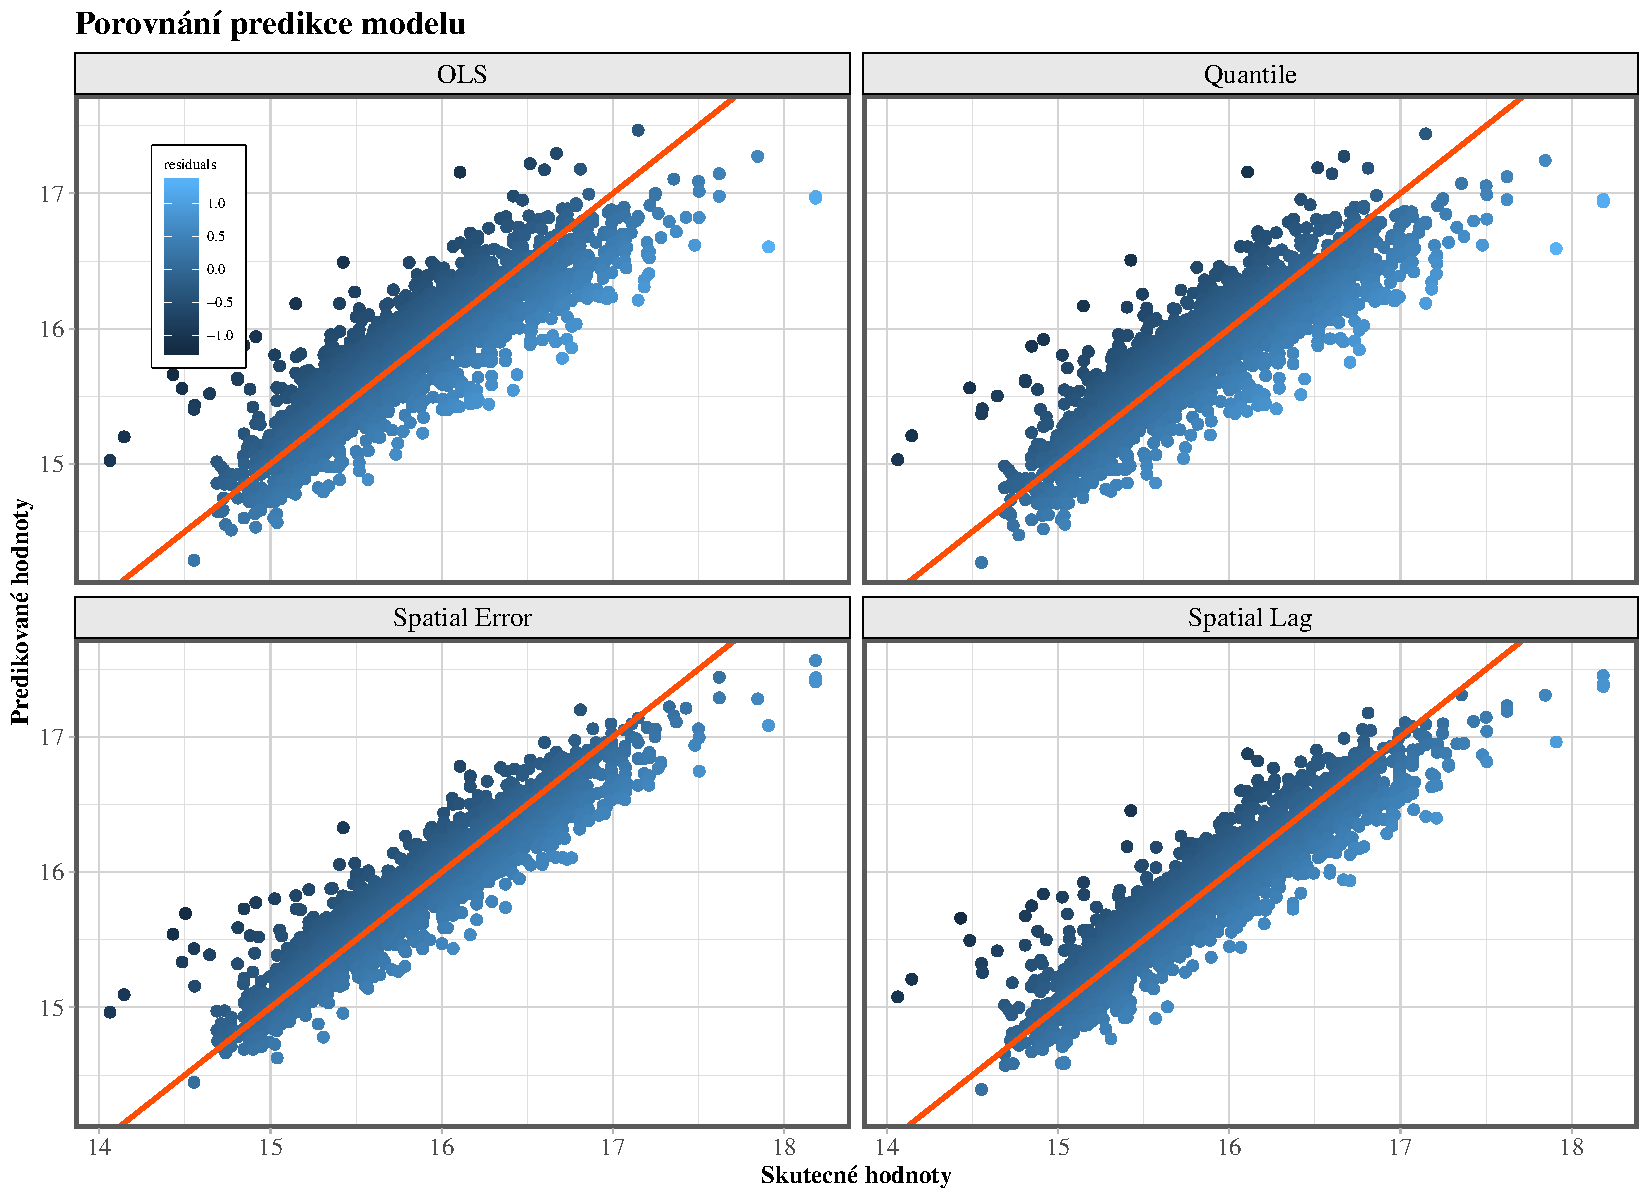
\includegraphics[width=1.1\textwidth]{flats_fitted.pdf}}
\caption{Porovnání skutečných a predikovaných hodnot}
\label{Porovnání skutečných a predikovaných hodnot}
\end{figure}

Vidíme, že hodnoty modelu \textit{Spatial Error} jsou nejvíce sblížené s linií 45 stupňů, tedy přímkou kde skutečné a predikované hodnoty jsou zcela totožné.

Dle základě regresní tabulky \ref{modely tabulka}, dále také dle metrik užitých v tabulce \ref{Metriky modelů} a nakonec dle predikcí na obrázku \ref{Porovnání skutečných a predikovaných hodnot} volíme \textit{Spatial Error model} pro statistickou inferenci.

V další části práce se budeme zabývat citlivostí vůči změnám speficikace relace sousednosti a citlivosti koeficientů v závislosti na matici \textit{W}.
\clearpage

\section{Citlivost na změny relace sousednosti}

V návaznosti na studii \cite{formanek2016stability} provedeme i my ověření stability koeficientů v závislosti na formulaci matice \textit{W}. Budeme nadále uvažovat relaci sousednosti dle \textit{K-nejbližších sousedů}, ale budeme ověřovat citlivost koeficientů pro různé hodnoty \textit{k}. Hlavním důvodem proč volíme algoritmus \textit{K-nejbližších sousedů} je skutečnost, že naše data nejsou rovnoměrně zastoupená v prostoru. pokud bychom např. volili metodiku \textit{do maximální vzdálenosti} mohlo by se stát, že některé jednotky budou mít mnohonásobně větší počet jednotek, které jsou definované jako sousedící. 

Pokud užíváme algoritmu \textit{K-nejbližších sousedů} nebude případné zkreslení způsobené distribucí dat nakolik výrazné. Dalším důvodem je výpočetní čas. U jednotlivých prostorových modelů popisujeme, že řešení není k dispozici v analytickém tvaru a hledá se iteračně, je patrné, že pokud pracujeme s maticí \textit{W}, která má v našem případě rozměr \textit{$2984 \times 2984$} je patrné, že výpočetní náročnost na hardware počítače je značná.

Citlivost koeficientů pro různé hodnoty počtu sousedních jednotek (v našem případě od 1 do 15 jednotek) je možné sledovat na obrázku \ref{Citlivost koeficientů v změny matice} níže.

\begin{figure}[ht]
\centering
\noindent\makebox[\textwidth]{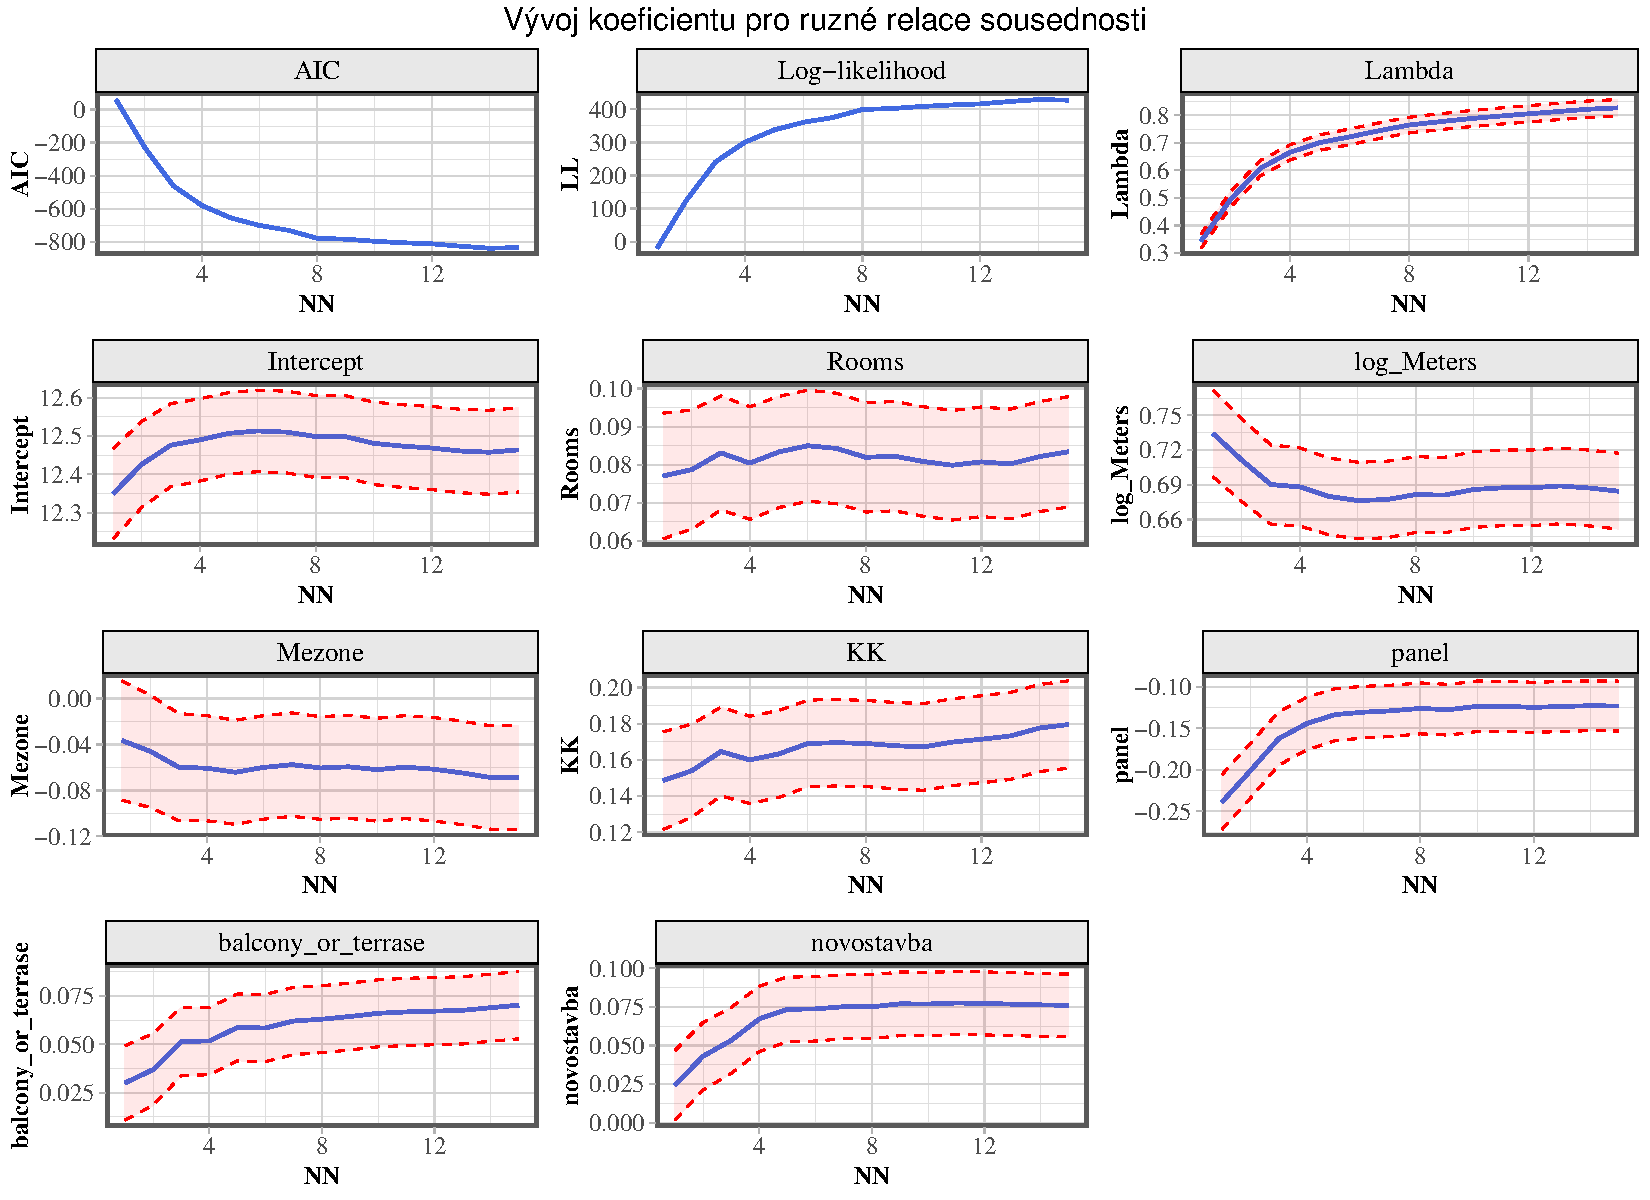
\includegraphics[width=1.11\textwidth]{spatial_sensiv.pdf}}
\caption{Citlivost koeficientů v změny matice \textit{W}}
\label{Citlivost koeficientů v změny matice}
\end{figure}

\clearpage

V našem případě je patrné, že hodnota, která minimalizuje hodnotu informačního kritéria je \textit{$k = 15$}, tento model také skutečně uvádíme v tabulce \ref{modely tabulka} a využíváme jej k výsledné statistické inferenci a zhodnocení stanovených hypotéz.


\section{Distribuce reziduí v prostoru}

OLS model není zcela kvalitní na oceňování nemovitostí na Pražském trhu, neboť nebere v potaz prostorové závislosti. Nicméně rezidua modelu mohou resp. jejich rozmístění v prostoru může představovat zajímavý indikátor.


Nejdříve spočítáme procentuální chyby predikce z modelu jednoduché regrese (bez \textit{Clusterů}) pro každé pozorování a následně dle intervalů hodnoty diskretizujeme.

Při pohledu na \ref{Shluková analýza reziduí} níže vidíme, že nemovistosti vyskytující se v historickém centru Prahy (Staroměstské náměstí a přilehlé okolí).

Ceny nemovistostí jsou zde více jak dvojnásobné (více jak 100\% rozdíl predikce) čistě z důvodů výskytů nemovistostí v historické části. Abychom tuto nevyrovnanost v reziduích odstranili, bylo by nutné každé nemovitosti v tomto centru přidat novu kontrolní proměnnou $\textit{Historické centru}$, která by nabývala hodnoty 1, pro nemovitosti v $\textit{Honosném Clusteru}$. Užití modelů bez prostorové závislosti nám umožňuje takovéto clustery identifikovat.

\clearpage
\begin{figure}[ht]
\centering
\noindent\makebox[\textwidth]{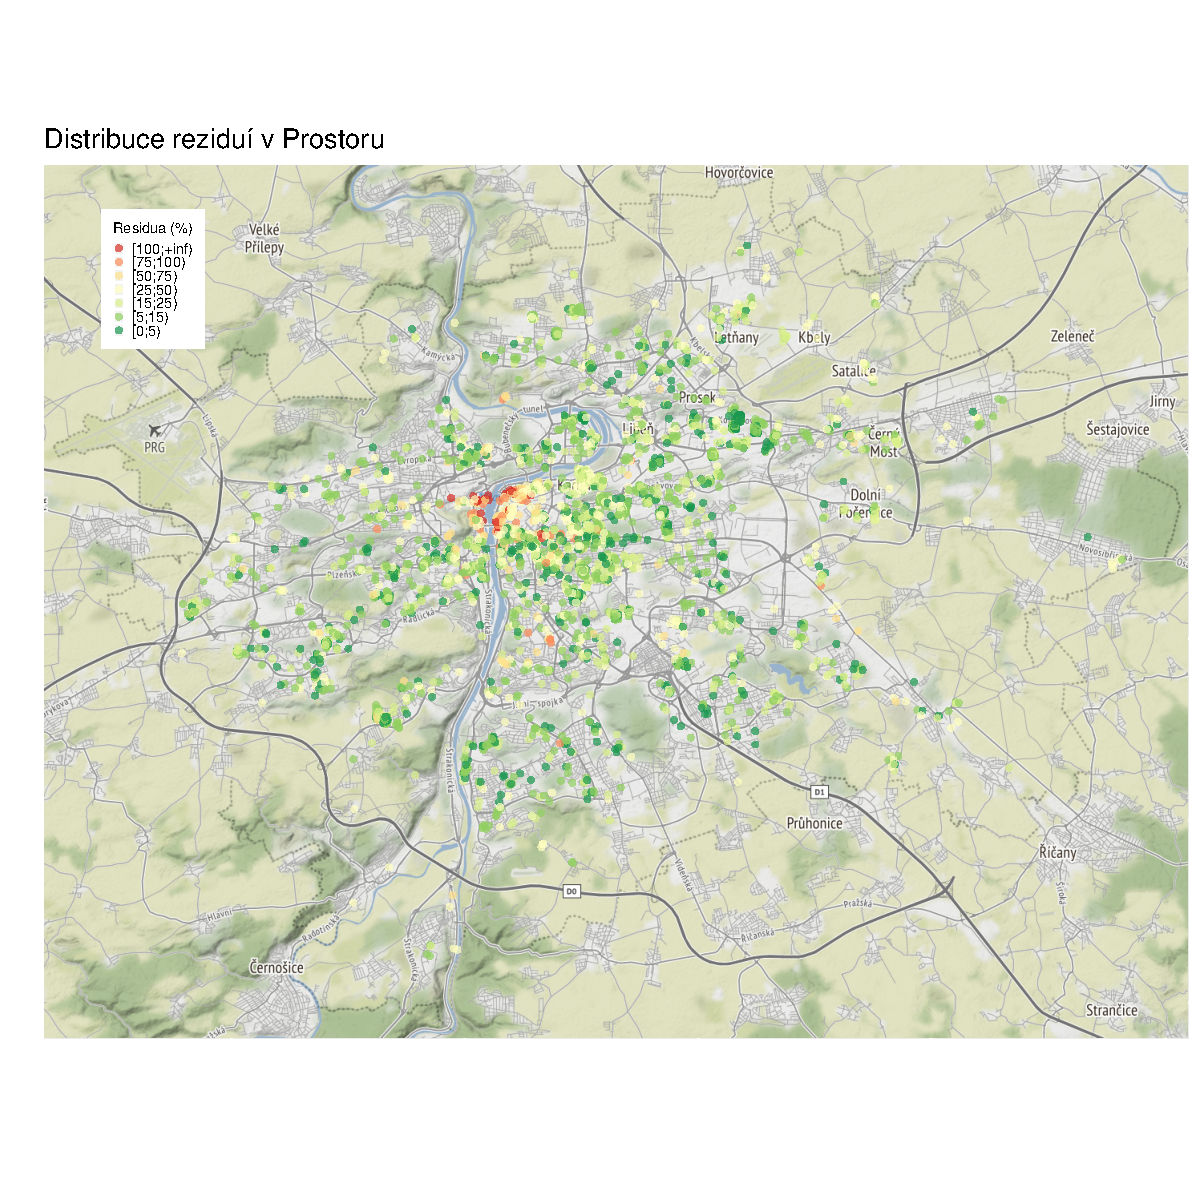
\includegraphics[width=1.2\textwidth]{flats_resid.pdf}}
\caption{Shluková analýza reziduí}
\label{Shluková analýza reziduí}
\end{figure}



\clearpage

\section{Závěr}

Na závěr naší studie se vrátíme zpět k našim stanovených hypotézám. Nejdříve jsme uvažovali, že prostorové modely z důvodu prostorové autokorelace disponují lepší predikční schopností a také lepším zachycením DGP. Tedy naší první stanovenou hypotézu lze na základě zjištění v této studii \textit{potvrdit}.

Dále jsme uvažovali identifikaci honosných Clusterů v Pražském trhu. Hlavním ukazatelem může být distribuce reziduí z lineárního modelu, který nebere v potaz prostorovou závislost. Na obrázku \ref{Shluková analýza reziduí} vidíme výrazný \textit{Honosný Cluster} v historické části Prahy. 

Takto identifikované clustery mohou mít relevantní informační hodnotu pro realitní agenty, pro obyvatelé, které o investici do nemovitosti uvažují a zejména pro majitelé nemovitostí, kteří uvažují o prodeji či pronájmu. 

Pokud se jejich nemovitost nachází v takovémto honosném Clusteru, lze cenu nemovitosti výrazně navýšit a očekávat i tak uzavření obchodu.

K poslední stanovené hypotéze, zda novostavba relevantně zvyšuje nemovitosti využijeme \textit{Spatia l Error modelu}. Parametr \textit{novostavby} je jak v tabulce \ref{modely tabulka}, tak také na \ref{Citlivost koeficientů v změny matice} vždy statisticky odlišný od hodnoty $0.$ Dle koeficientu u našeho modelu odhadujeme, že mezní efekt nemovitosti je roven zhruba 7.5 \%, tedy opět \textit{potvrzujeme} naši stanovenou hypotézu.


Naše Studie představuje aplikaci prostorových modelů na trhu pražských nemovitostí. Z důvodu prostorové autokorelace jsou prostorové modely pro takový typ datového souboru vhodné a jejich uplatnění v praxi stále roste. V budoucím výzkumu lze dataset rozšířit o rozměr času a jednotlivé analýzy provádět nikoliv, jako na průřezových datech, ale na datech panelových.






\clearpage
\section{Přílohy} \label{Přílohy}

\begin{figure}[ht]
\centering
\noindent\makebox[\textwidth]{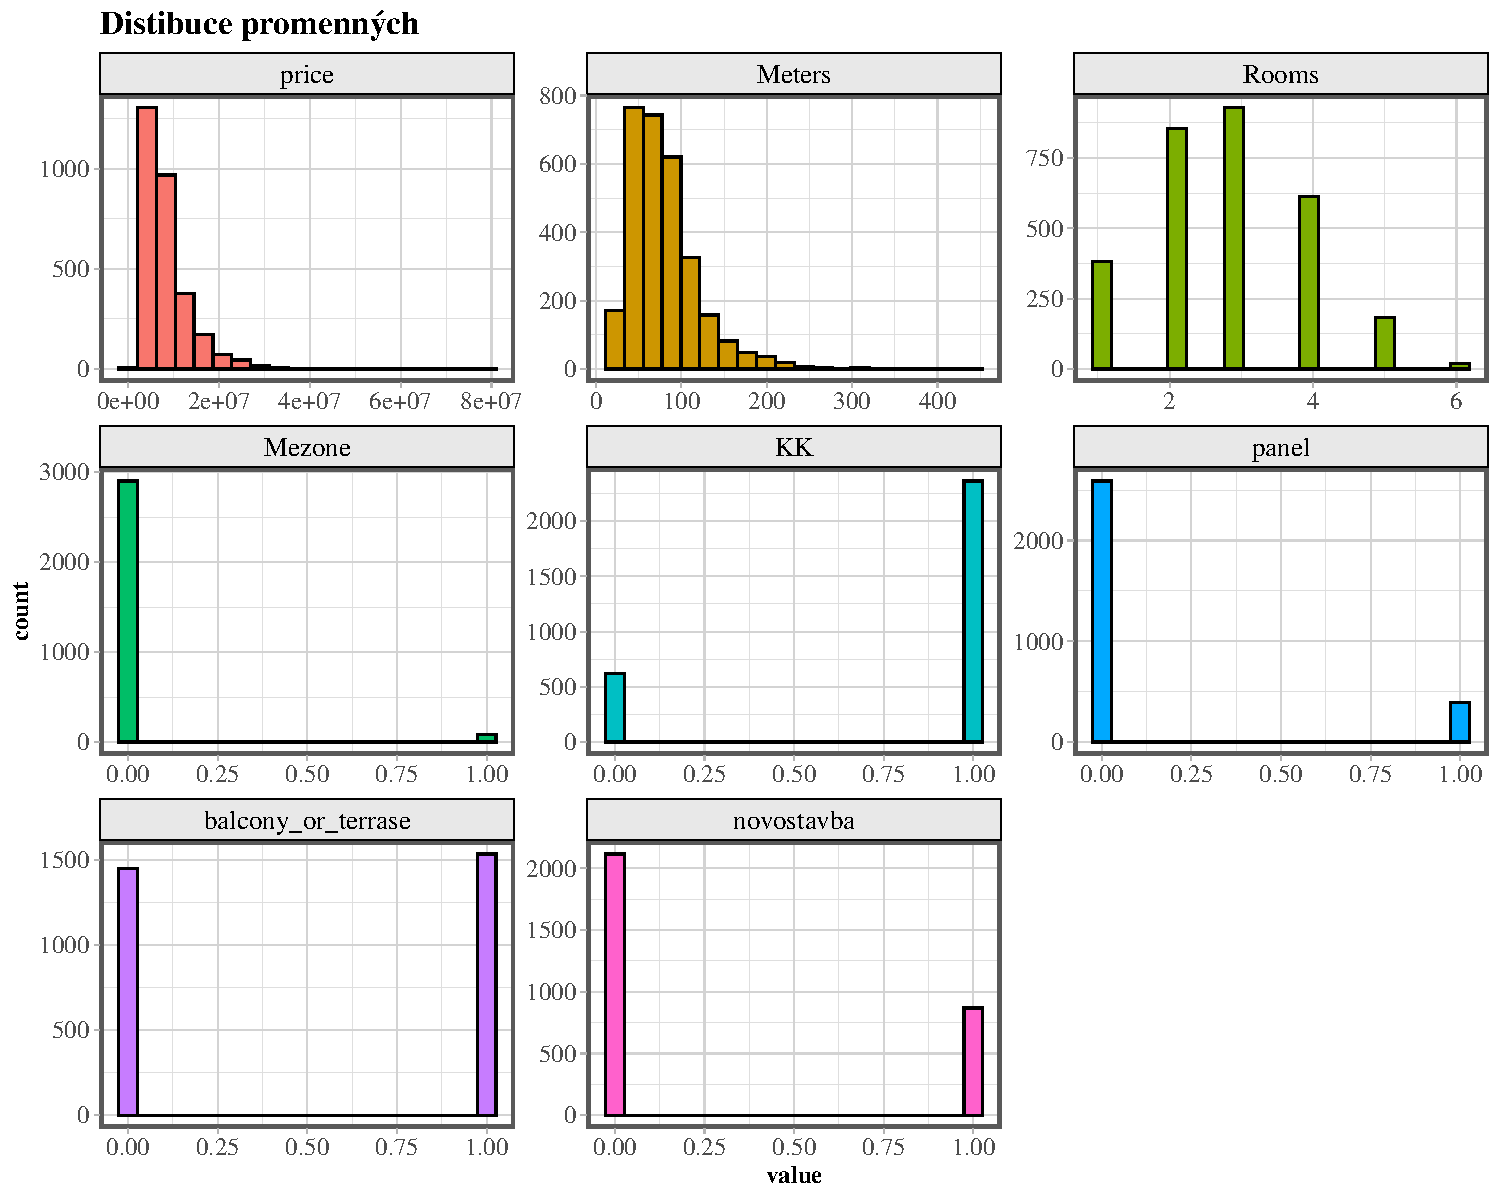
\includegraphics[width=1.1\textwidth]{datahist.pdf}}
\caption{Distribuce Proměnných}
\label{Distribuce Proměných}
\end{figure}

\clearpage

\begin{figure}[ht]
\centering
\noindent\makebox[\textwidth]{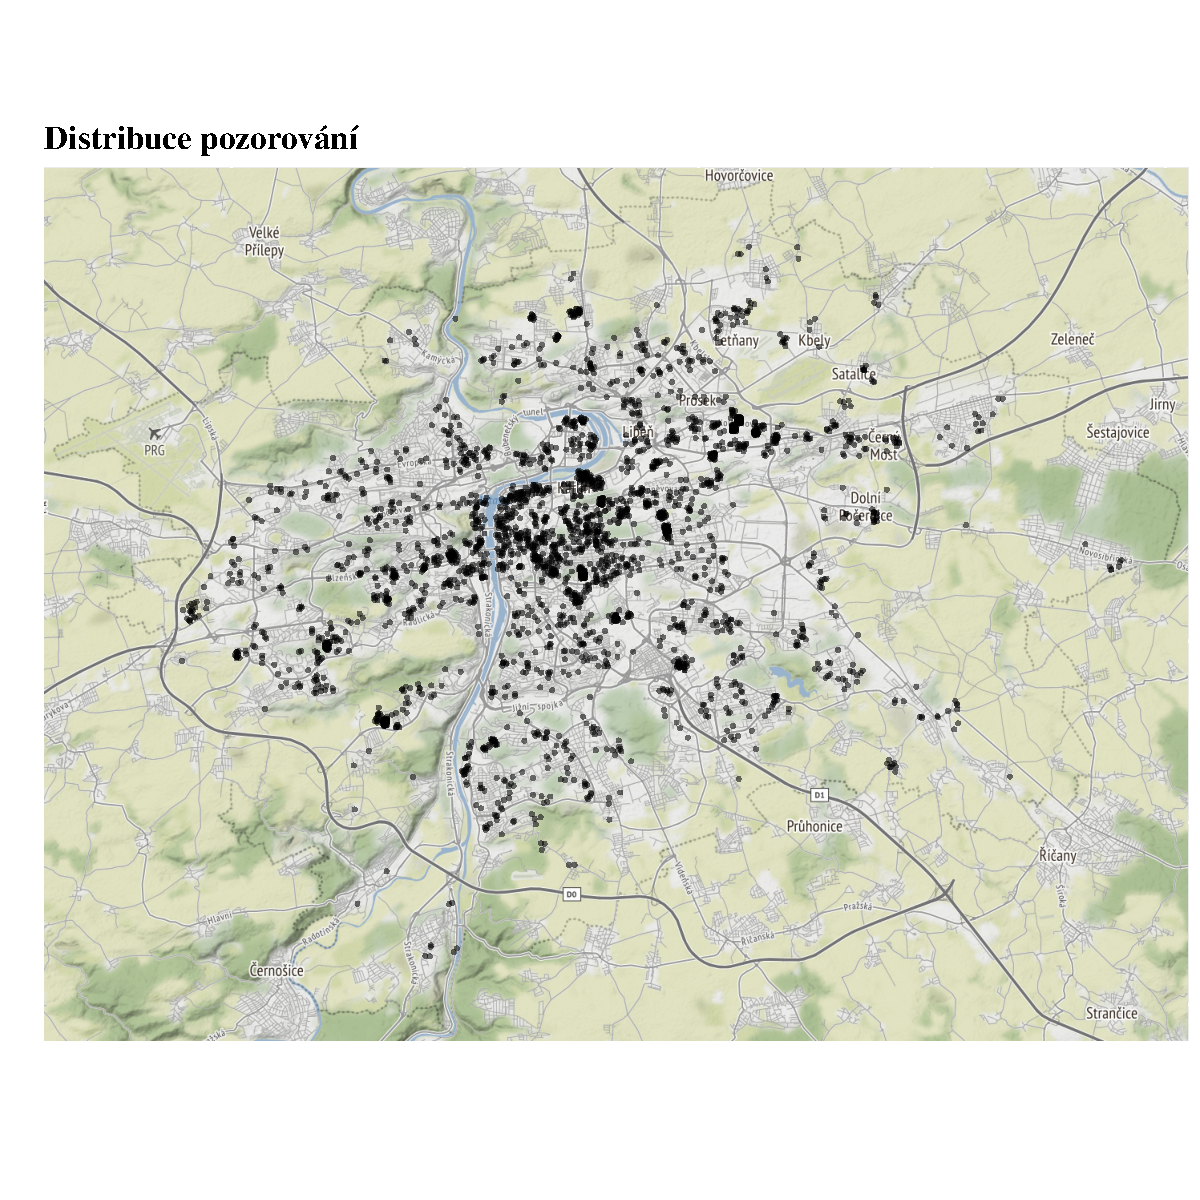
\includegraphics[width=1.1\textwidth]{flats.pdf}}
\caption{Distribuce Pozorování v prostoru}
\label{Distribuce pozorování v prostoru}
\end{figure}

\clearpage

\begin{figure}[ht]
\centering
\noindent\makebox[\textwidth]{\includegraphics[width=1.1\textwidth]{flat_cluster.pdf}}
\caption{Distribuce Pozorování a Clusterování}
\label{Distribuce Pozorování a Clusterování}
\end{figure}

\clearpage

\begin{figure}[ht]
\centering
\noindent\makebox[\textwidth]{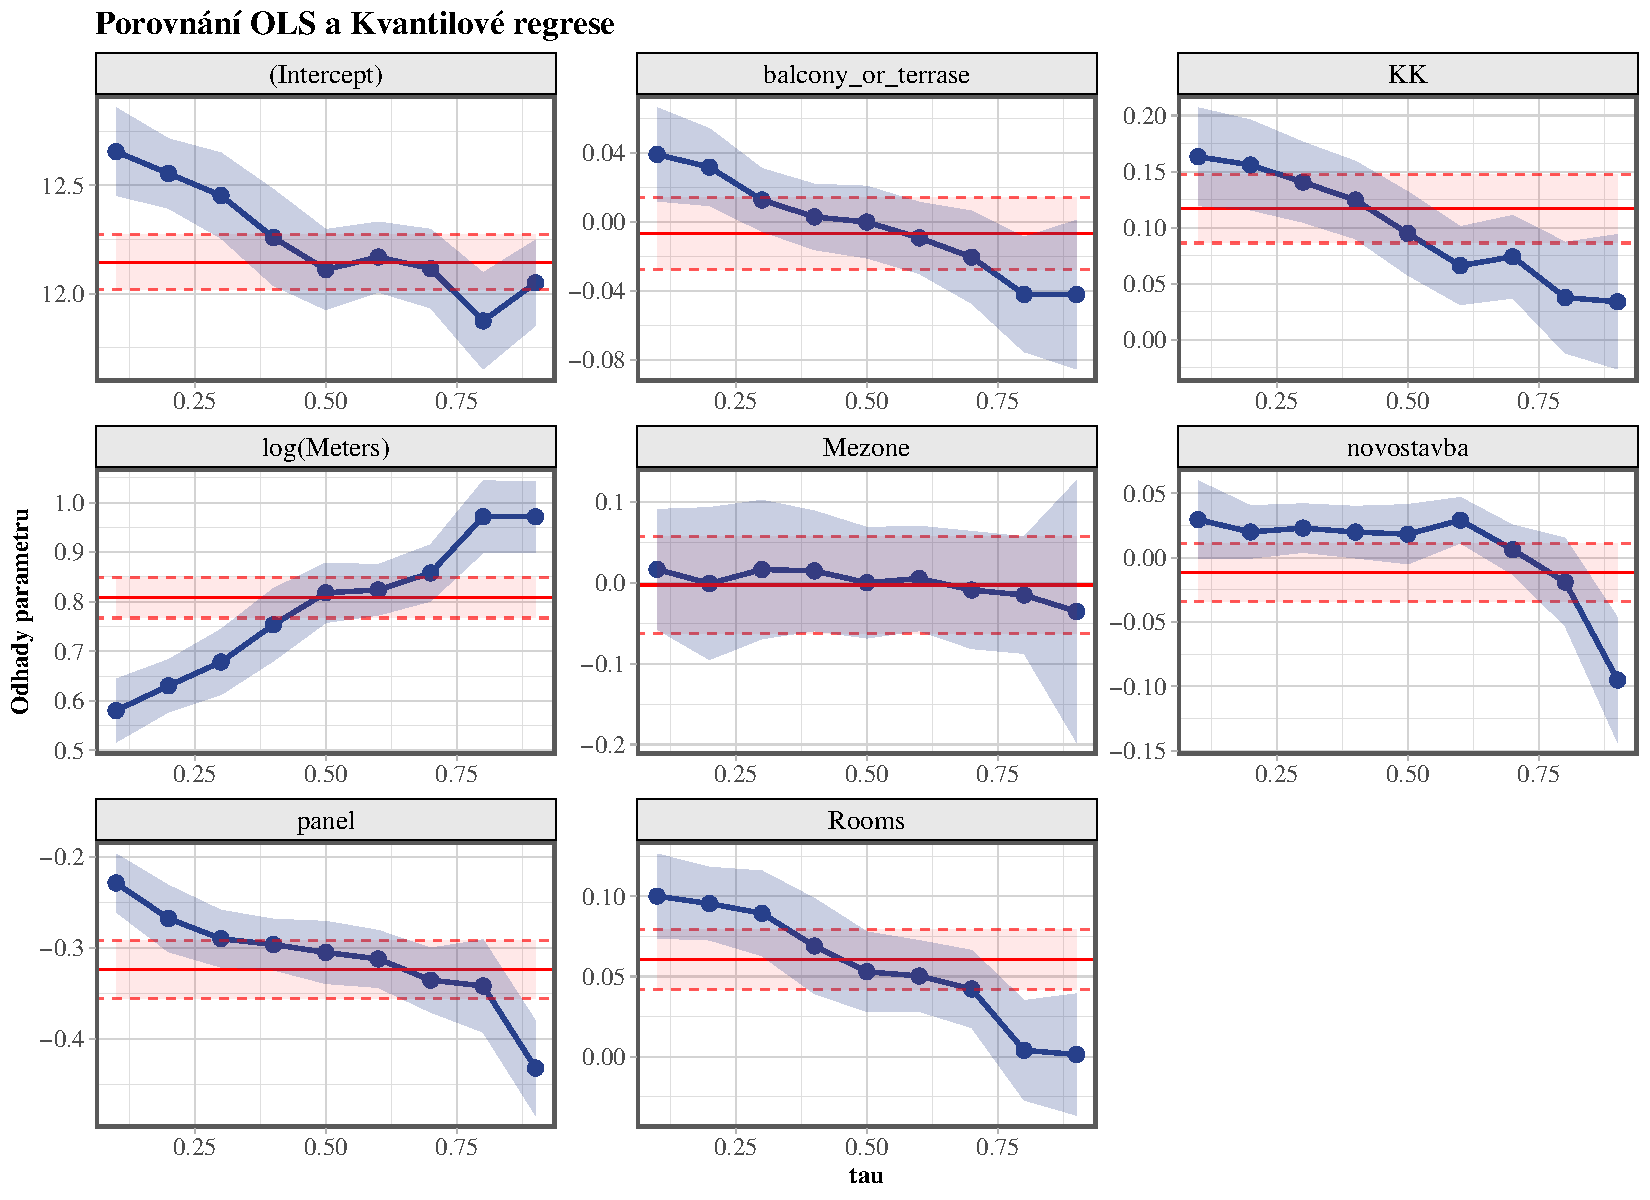
\includegraphics[width=1.1\textwidth]{kvant.pdf}}
\caption{Citlivost Kvantilové regrese}
\label{Citlivost kvantilové regrese}
\end{figure}

%%%%%%%%%%%%%%%%%%%%%%%%%%%%%%
  \clearpage
%
% PRO VLOZENI CITACI A REFERENCI
\bibliographystyle{apacite}
\newpage
\bibliography{liter}
%%%%%%%%%%%%%%%%%%%%%%%%%%%%%%%
\end{document}
